\subsection{Rf} \label{sec:ontwerp:Rf}
Nadat de pH waarde gemeten is, moet deze worden opgestuurd door middel van een draadloze verbinding. Dit word gedaan door het RF blok. Het RF blok bevindt zich, zoals te zien in \cref{fig:RFInSchema}, na de digitale signaalverwerking, en is het laatste blok in het systeem van de sensormodule.
\begin{figure}[!htbp]
    \centering
    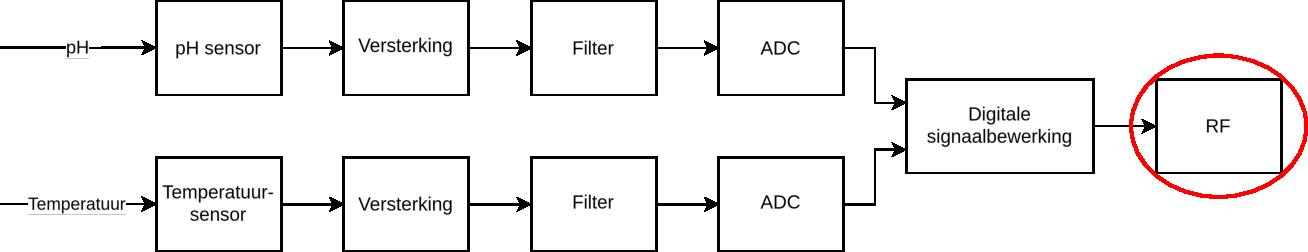
\includegraphics[width=0.95\textwidth]{signaalblokjes/RFInSchema}
    \caption{Waar de RF zich bevind in het blokschema van de signaalverwerking in \cref{fig:analogeBewerkingsFunctie}.}
    \label{fig:RFInSchema}
\end{figure}

In \cref{sec:systemSpecifications} is aangegeven dat het ontvangst systeem gebruik maakt van een \mcu. Om te kunnen berekenen wat het minimale zendvermogen van de sensormodule moet zijn, moet de noise figure (NF) van de \mcu worden bepaald. De NF van de \mcu wordt gebruikt om de ontvangstgevoeligheid te bepalen. Deze ontvangstgevoeligheid wordt gebruikt om het minimale zendvermogen te berekenen.

In de datasheet van de \mcu is de ontvangst gevoeligheid gegeven. Bij een datasnelheid van 1 Mbit/s, een bit error ratio (BER) van  $1 \times 10^{-3}$ en gaussian frequency shift keying (GFSK) modulatie, is de ontvangstgevoeligheid van de \mcu$\,$-96 dBm \cite{nrf52810}.

Om de NF van de \mcu te berekenen moet eerst de minimaal benodigde SNR worden berekend. De minimaal benodigde SNR is het gevolg van een gespecificeerde BER en kan worden berekend met \cref{eq:minSNRbasedonPe}. $P_E$ is gelijk aan de BER in het geval er een significante hoeveelheid bit errors hebben plaatsgevonden \cite{BERtoPe}. De $\SNR_{min}$ van de \mcu komt uit op 5.17 dB.
\begin{equation}\label{eq:minSNRbasedonPe}
    SNR_{min}=\sqrt{2}\inverfc\left(2P_E\right)
    \tagaddtext{[\si{\decibel}]}
\end{equation}

Met een bekende $SNR_{min}$ is het mogelijk om de NF van de \mcu te berekenen met \cref{eq:calcNRF52810NF}, in het geval er alleen uit wordt gegaan van thermische ruis \cite{SWRA030}. $N_0$ is het thermische ruisvermogen per Hz en kan met $N_0=kT_0$ worden berekend, hierbij is k de constante van Boltzmann en $T_0=290$ Kelvin \cite{Short-rangeWirelessCommunication}. $B$ is de datasnelheid in bits/s en $S_r$ is de ontvangstgevoeligheid. Voor de \mcu komt dit uit op 26 dB.
\begin{equation}\label{eq:calcNRF52810NF}
    % NF_{r}=S_r-10\left(\log\left(N_0\right)+\log\left(B\right)\right)-SNR_{min}
    NF_r=20\log\left(\frac{S_{r}}{N_0B\,\SNR_{min}}\right)
    \tagaddtext{[\si{\decibel}]}
\end{equation}

% Met BER/Pe ontvangersgevoeligheid berekenen
\Cref{eq:calcReceiverSensitivity} kan gebruikt worden om de ontvangst gevoeligheid te berekenen van de ontvanger. Omdat de NF van de \mcu berekend is, is het nu mogelijk om de ontvangstgevoeligheid van de \mcu te berekenen voor een gegeven BER. In hoofdstuk \ref{sec:systemSpecifications} is een minimale BER van $1\times10^{-5}$ voor de draadloze communicatie gespecificeerd. In de datasheet staat dat de \mcu gebruik maakt van GFSK modulatie \cite{nrf52810}. Het is hiermee mogelijk om de minimale ontvangst \SNR te berekenen voor een BER van $1\times10^{-5}$. Deze komt uit op 12.6 dB.

Wanneer er  bij het berekenen van de ontvangst gevoeligheid naast de thermische ruis ook het achtergrond vermogen van andere zenders wordt meegenomen, moet bij $N_0$ een constante ($\Delta N)$ worden opgeteld. $\Delta N$ is afhankelijk van de omgeving van de sensormodule. De sensormodule die in dit project wordt ontworpen moet in een industriële omgeving kunnen werken. Uit \cite{kumar2020spectrum} is te halen dat in een dergelijke omgeving een $\Delta N$ van $-105\,\,\si{\deci\belmilliwatt\,\hertz^{-1}}$ een redelijke waarde is. Uit \cref{eq:calcReceiverSensitivity} volgt dat de ontvangstgevoeligheid \qty{-57}{\deci\belmilliwatt} wordt ingeval van een bandbreedte van $\SI{1}{\mega\hertz}$. Met een bandbreedte van $\SI{2}{\mega\hertz}$ is de ontvangstgevoeligheid \qty{-54}{\deci\belmilliwatt}.
\begin{equation}\label{eq:calcReceiverSensitivity}
    S_r=\left(N_0+\Delta N\right)BF_T \SNR_{min}
    \tagaddtext{[\si{\deci\belmilliwatt}]}
\end{equation}

% Minimaal zendvermogen berekenen
Om het minimale zendvermogen te bepalen moet ook berekend worden hoeveel signaalverlies er optreed door path loss. Hiervoor moet de afstand tussen de antennes bekend zijn. Daarnaast moet ook de hoogte van beide antennes ten opzichte van de grond bekend zijn. Met het meest complete path loss model uit \cite{determineFittingsCoef}
\footnote{Bron \cite{determineFittingsCoef} is in \cref{ap:determineFittingsCoef} te zien.}
is op basis van de gegevens uit \cref{tab:gegevensCalcPathLoss} berekend dat er 53.2 dB aan path loss optreed.
\begin{table}[!htbp]
    \centering
    \begin{tabular}{l|l}
        Hoogte antenne 1                    & $\qty{1  }{\meter}$               \\\hline
        Hoogte antenne 2                    & $\qty{1  }{\meter}$               \\\hline
        Antenne 1 gain                      & $\qty{2.5}{\decibel i}$           \\\hline
        Antenne 2 gain                      & $\qty{2.5}{\decibel i}$           \\\hline
        Afstand tussen de antennes          & $\qty{10 }{\meter}$               \\\hline
        Grond permeabiliteit $\epsilon_r$   & $\qty{3.4}{\henry\,\meter^-1}$    \\\hline
        Fittingscoëfficiënt $l_f$           & 7.8                               \\\hline
        zendfrequentie                      & $\qty{2.4}{\giga\hertz}$
    \end{tabular}
    \caption{De aannames voor het berekenen van de path loss}
    \label{tab:gegevensCalcPathLoss}
\end{table}
% \begin{itemize}
%     \item Hoogte antenne 1, 1 meter is
%     \item Hoogte antenne 2, 1 meter is
%     \item Gain antenne 1,  2.5 dBi is
%     \item Gain antenne 2,  2.5 dBi is
%     \item Afstand tussen de antennes 10 meter is
%     \item De grond permeabiliteit 3.4 is
%     \item De fittingscoëfficiënt $l_f$ 7.8 is
%     \item De zendfrequentie 2.4G Hz
% \end{itemize}

Omdat de ontvangstgevoeligheid en het signaalverlies ten gevolge van path loss bekend zijn, is het mogelijk om een minimum zendvermogen te berekenen. Dit minimale zendvermogen kan met \cref{eq:minTransmitPower} berekend worden. Dit komt uit op \qty{-4}{\deci\belmilliwatt} in geval van een bandbreedte van $\SI{1}{\mega\hertz}$. Indien de bandbreedte $\SI{2}{\mega\hertz}$ is, is het minimum zendvermogen \qty{-1}{\deci\belmilliwatt}.
\begin{equation}\label{eq:minTransmitPower}
    P_{z,min}= 10\log\left(S_r\right) + PL
    \tagaddtext{[\si{\deci\belmilliwatt}]}
\end{equation}

Om een inschatting te kunnen maken of het beter is om met een bandbreedte van 1 of $\SI{2}{\mega\hertz}$ te zenden moet er gekeken worden welke van de twee het meest efficient is. Dit kan gedaan worden door te berekenen hoeveel energie het kost om een datapakket te versturen. Hiervoor kan \cref{eq:calcPperPacket} worden gebruikt. $DR$ is de datasnelheid in bits per seconden, $l$ is de lengte van een datapakket in bits en $P_{z,min}$ is het minimaal benodigde zendvermogen in Watt. De lengte van een pakket is 37 bytes. Dit zorgt er voor dat per pakket 296 bits moeten worden verzonden. Door \cref{eq:calcPperPacket} te gebruiken kan nu berekend worden dat het \qty{117.8}{n\joule} kost om met een bandbreedte van $\SI{1}{\mega\hertz}$ een pakket te verzenden en dat het \qty{117.6}{n\joule} kost om met een bandbreedte van $\SI{2}{\mega\hertz}$ een pakket te verzenden. Het verschil in de hoeveelheid energie die nodig is om op $\SI{1}{\mega\hertz}$ dan wel $\SI{2}{\mega\hertz}$ te zenden is verwaarloosbaar klein. Om ervoor te zorgen dat er voor een zo kort mogelijke tijd wordt gezonden is het aan te raden om met een bandbreedte van $\SI{2}{\mega\hertz}$ te zenden.
\begin{equation}\label{eq:calcPperPacket}
    E_{zp}=\frac{l}{DR}P_{z,min}
    \tagaddtext{[\si{\joule}]}
\end{equation}

Om in te schatten hoeveel het draadloos zenden over tijd kost kan \cref{eq:calcRfAvaragePower} gebruikt worden als indicatie. In \cref{eq:calcRfAvaragePower} is $f_{zp}$ de frequentie waarmee er data pakketten wordt gestuurd. Hiermee is berekend dat het minimale zendvermogen over tijd \qty{7.1}{\micro\watt} is.
\begin{equation}\label{eq:calcRfAvaragePower}
    \overline{P_{z}}=E_{zp}f_{zp}
    \tagaddtext{[\si{\watt}]}
\end{equation}



% modulatie
% Path loss
% min vermogen ?
% communicatie protocol